\documentclass{beamer}
\usepackage[english]{babel}
\usepackage{unicode-math}
\usepackage{xunicode}
\usepackage{url}
\usepackage{cite}
\usepackage{graphicx}
\usepackage[justification=centering, labelfont=bf]{caption}
\usepackage{float}
\usepackage{pgfgantt}
\usepackage{marvosym}
\usepackage{siunitx}
\usepackage{multirow}
\usepackage{svg}
\usetheme{Antibes}
\setbeamertemplate{navigation symbols}{}
\captionsetup[figure]{labelformat=empty}
\setcounter{tocdepth}{1}
\title{Platform for massive multiplayer programming games}
\institute{Facultat d'Informàtica de Barcelona}
\author{Héctor Ramón Jiménez}
\date{January 28, 2016}
\begin{document}
\frame{\titlepage}
\begin{frame}{Overview}
\tableofcontents
\end{frame}
\section{Introduction}
\subsection{Programming games}
\begin{frame}{What is a programming game?}
...
\end{frame}
\section{Formulation}
\subsection{Analysis}
\begin{frame}{The problem}
...
\end{frame}
\begin{frame}{The state of the art}
...
\end{frame}
\subsection{Design}
\begin{frame}{The solution}
...
\end{frame}
\section{Planning}
\subsection{Time plan}
\begin{frame}{Time table}
...
\end{frame}
\begin{frame}{Time line}
...
\end{frame}
\subsection{Budget}
\begin{frame}{Total budget}
...
\end{frame}
\section{Implementation}
\subsection{Methodology}
\begin{frame}{Continuous integration}
...
\end{frame}
\subsection{The first prototype}
\begin{frame}{A simple prototype}
...
\end{frame}
\begin{frame}{The engine architecture}
\begin{figure}[H]
\begin{center}
\noindent\resizebox{\textwidth}{!}{
\begin{tikzpicture}[->,>=stealth',shorten >=1pt,auto,node distance=0.8cm,
    main node/.style={thick,circle,draw,minimum width=2.5cm}]

    \node[main node] (1) {master};

	\node[auto=false] (2) [below=of 1]{\ldots};
    \node[auto=false] (21) [left=of 2]{};
    \node[auto=false] (23) [left=of 21]{};
    \node[auto=false] (22) [right=of 2]{};
    \node[auto=false] (24) [right=of 22]{};

    \node[main node] (3) [left=of 23]{worker$_1$};
    \node[main node] (4) [right=of 24]{worker$_N$};

    \node[auto=false] (5) [below=of 3]{\ldots};
    \node[main node] (6) [left=of 5]{player$_{1,1}$};
    \node[main node] (7) [right=of 5]{player$_{1,{M_1}}$};

    \node[auto=false] (8) [below=of 4]{\ldots};
    \node[main node] (9) [left=of 8]{player$_{N,1}$};
    \node[main node] (10) [right=of 8]{player$_{N,{M_N}}$};


    \path (1) edge (3);
    \path (1) edge (4);

    \path (3) edge (6);
    \path (3) edge (7);

    \path (4) edge (9);
    \path (4) edge (10);
\end{tikzpicture}

}
\end{center}
\caption{Hierarchy of engine processes with $N$ workers and $\sum_{i=1}^N M_i$ players}
\label{engine_arch}
\end{figure}
\end{frame}
\begin{frame}{The prototype result}
\begin{figure}[H]
\begin{center}
\noindent\resizebox{!}{15em}{
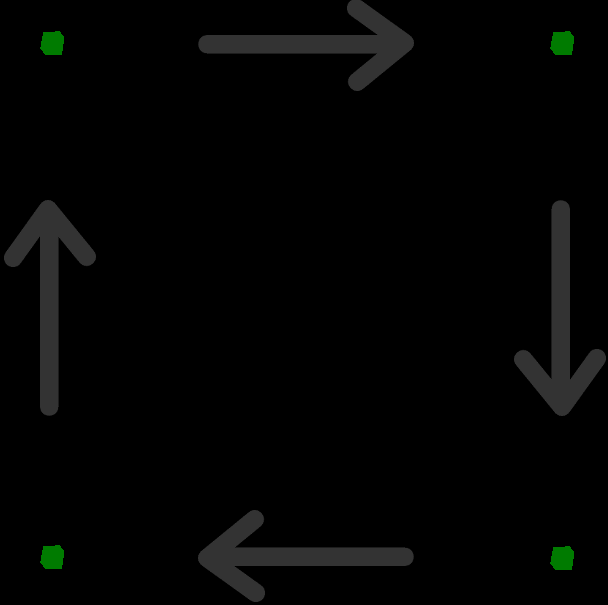
\includegraphics{images/cube_movement.png}
}
\end{center}
\caption{A cube that was moved by the player program}
\label{cube_movement}
\end{figure}
\end{frame}
\subsection{Continuous integration}
\begin{frame}{Continuous integration setup}
...
\end{frame}
\subsection{The log system}
\begin{frame}{Match replay}
...
\end{frame}
\begin{frame}{Event sourcing}
...
\end{frame}
\begin{frame}{Snapshots}
...
\end{frame}
\begin{frame}{Log compression}
...
\end{frame}
\subsection{Deployment of AI}
\begin{frame}{Authentication}
...
\end{frame}
\begin{frame}{Player login}
\begin{figure}[H]
\makebox[\textwidth]{
\noindent\resizebox{!}{180pt}{

\includegraphics{images/login_ok.png}
}
\noindent\resizebox{!}{180pt}{

\includegraphics{images/login_error.png}
}
}
\caption{Login form. Valid (left). Invalid (right)}
\label{login_form}
\end{figure}
\end{frame}
\begin{frame}{AI hot-swapping}
\begin{figure}[H]
\makebox[\textwidth]{
\noindent\resizebox{!}{180pt}{
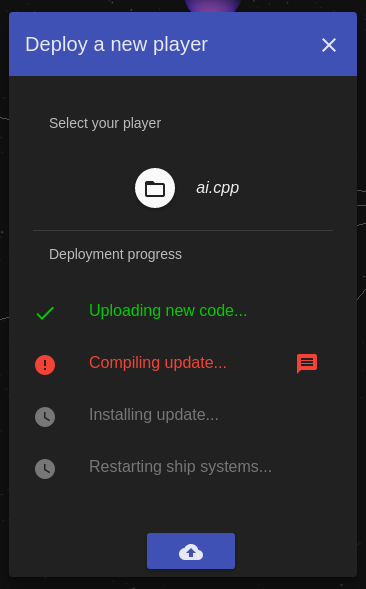
\includegraphics{images/deploy_error.png}
}
}
\caption{Player deployment with a compilation error}
\label{deploy_error}
\end{figure}
\end{frame}
\subsection{The first world}
\begin{frame}{Galcon and Planet Wars}
...
\end{frame}
\begin{frame}{Procedural generation of planetary systems}
...
\end{frame}
\subsection{Fleets and planets}
\begin{frame}{Game loop support}
...
\end{frame}
\subsection{A whole galaxy}
\begin{frame}{From a system to a galaxy}
...
\end{frame}
\section{Demonstration}
\begin{frame}{Space Wars}
...
\end{frame}
\section{Evaluation}
\subsection{Validation}
\begin{frame}{Stable and scalable}
...
\end{frame}
\subsection{Conclusion}
\begin{frame}{Summary}
...
\end{frame}
\begin{frame}{Final thoughts}
...
\end{frame}
\end{document}
